\documentclass[tikz,border=4pt]{standalone}
\usepackage{amsmath}
\begin{document}
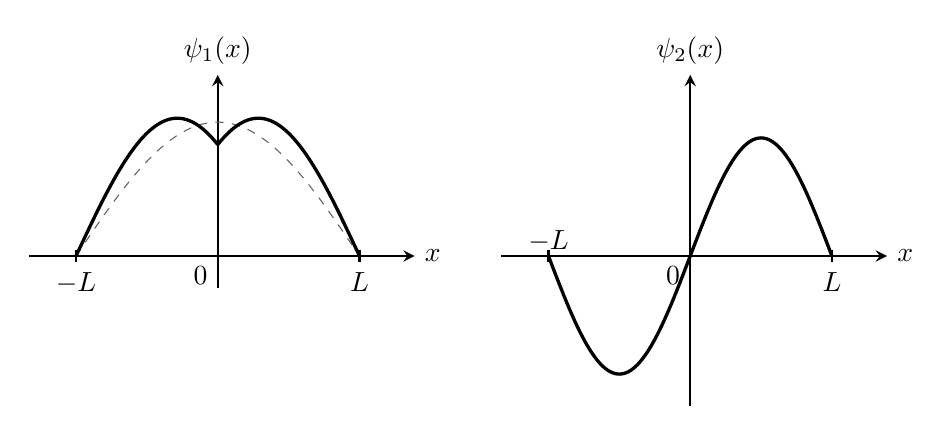
\begin{tikzpicture}[>=stealth, thick, scale=1.0]
  % Left: Ground state (even, cusp at x=0)
  \begin{scope}[xshift=0cm]
    \draw[->] (-2.4, 0) -- (2.5, 0) node[right] {$x$};
    \draw[->] (0, -0.4) -- (0, 2.3) node[above] {$\psi_1(x)$};
    \node[below left] at (0, 0) {$0$};
    \draw (-1.8, 0.08) -- (-1.8, -0.08) node[below] {$-L$};
    \draw (1.8, 0.08) -- (1.8, -0.08) node[below] {$L$};

    % V1 = 0 (dashed)
    \draw[dashed, thin, black!60, domain=-1.8:1.8, samples=80]
      plot (\x, {1.7 * cos(deg(pi*\x/3.6))});
    % V1 > 0 (solid with cusp at x=0: sin(k*(L-|x|)) with k*L = 2.3)
    \draw[very thick, domain=-1.8:0, samples=60]
      plot (\x, {1.75 * sin(deg(2.2*(1 + \x/1.8)))});
    \draw[very thick, domain=0:1.8, samples=60]
      plot (\x, {1.75 * sin(deg(2.2*(1 - \x/1.8)))});
  \end{scope}

  % Right: 1st excited state (odd, unchanged)
  \begin{scope}[xshift=6.0cm]
    \draw[->] (-2.4, 0) -- (2.5, 0) node[right] {$x$};
    \draw[->] (0, -1.9) -- (0, 2.3) node[above] {$\psi_2(x)$};
    \node[below left] at (0, 0) {$0$};
    \draw (-1.8, 0.08) -- (-1.8, -0.08) node[above] {$-L$};
    \draw (1.8, 0.08) -- (1.8, -0.08) node[below] {$L$};

    \draw[very thick, domain=-1.8:1.8, samples=100]
      plot (\x, {1.5 * sin(deg(pi*\x/1.8))});
  \end{scope}
\end{tikzpicture}
\end{document}
